\section{Harrison Armory Sherman}

\begin{center}
    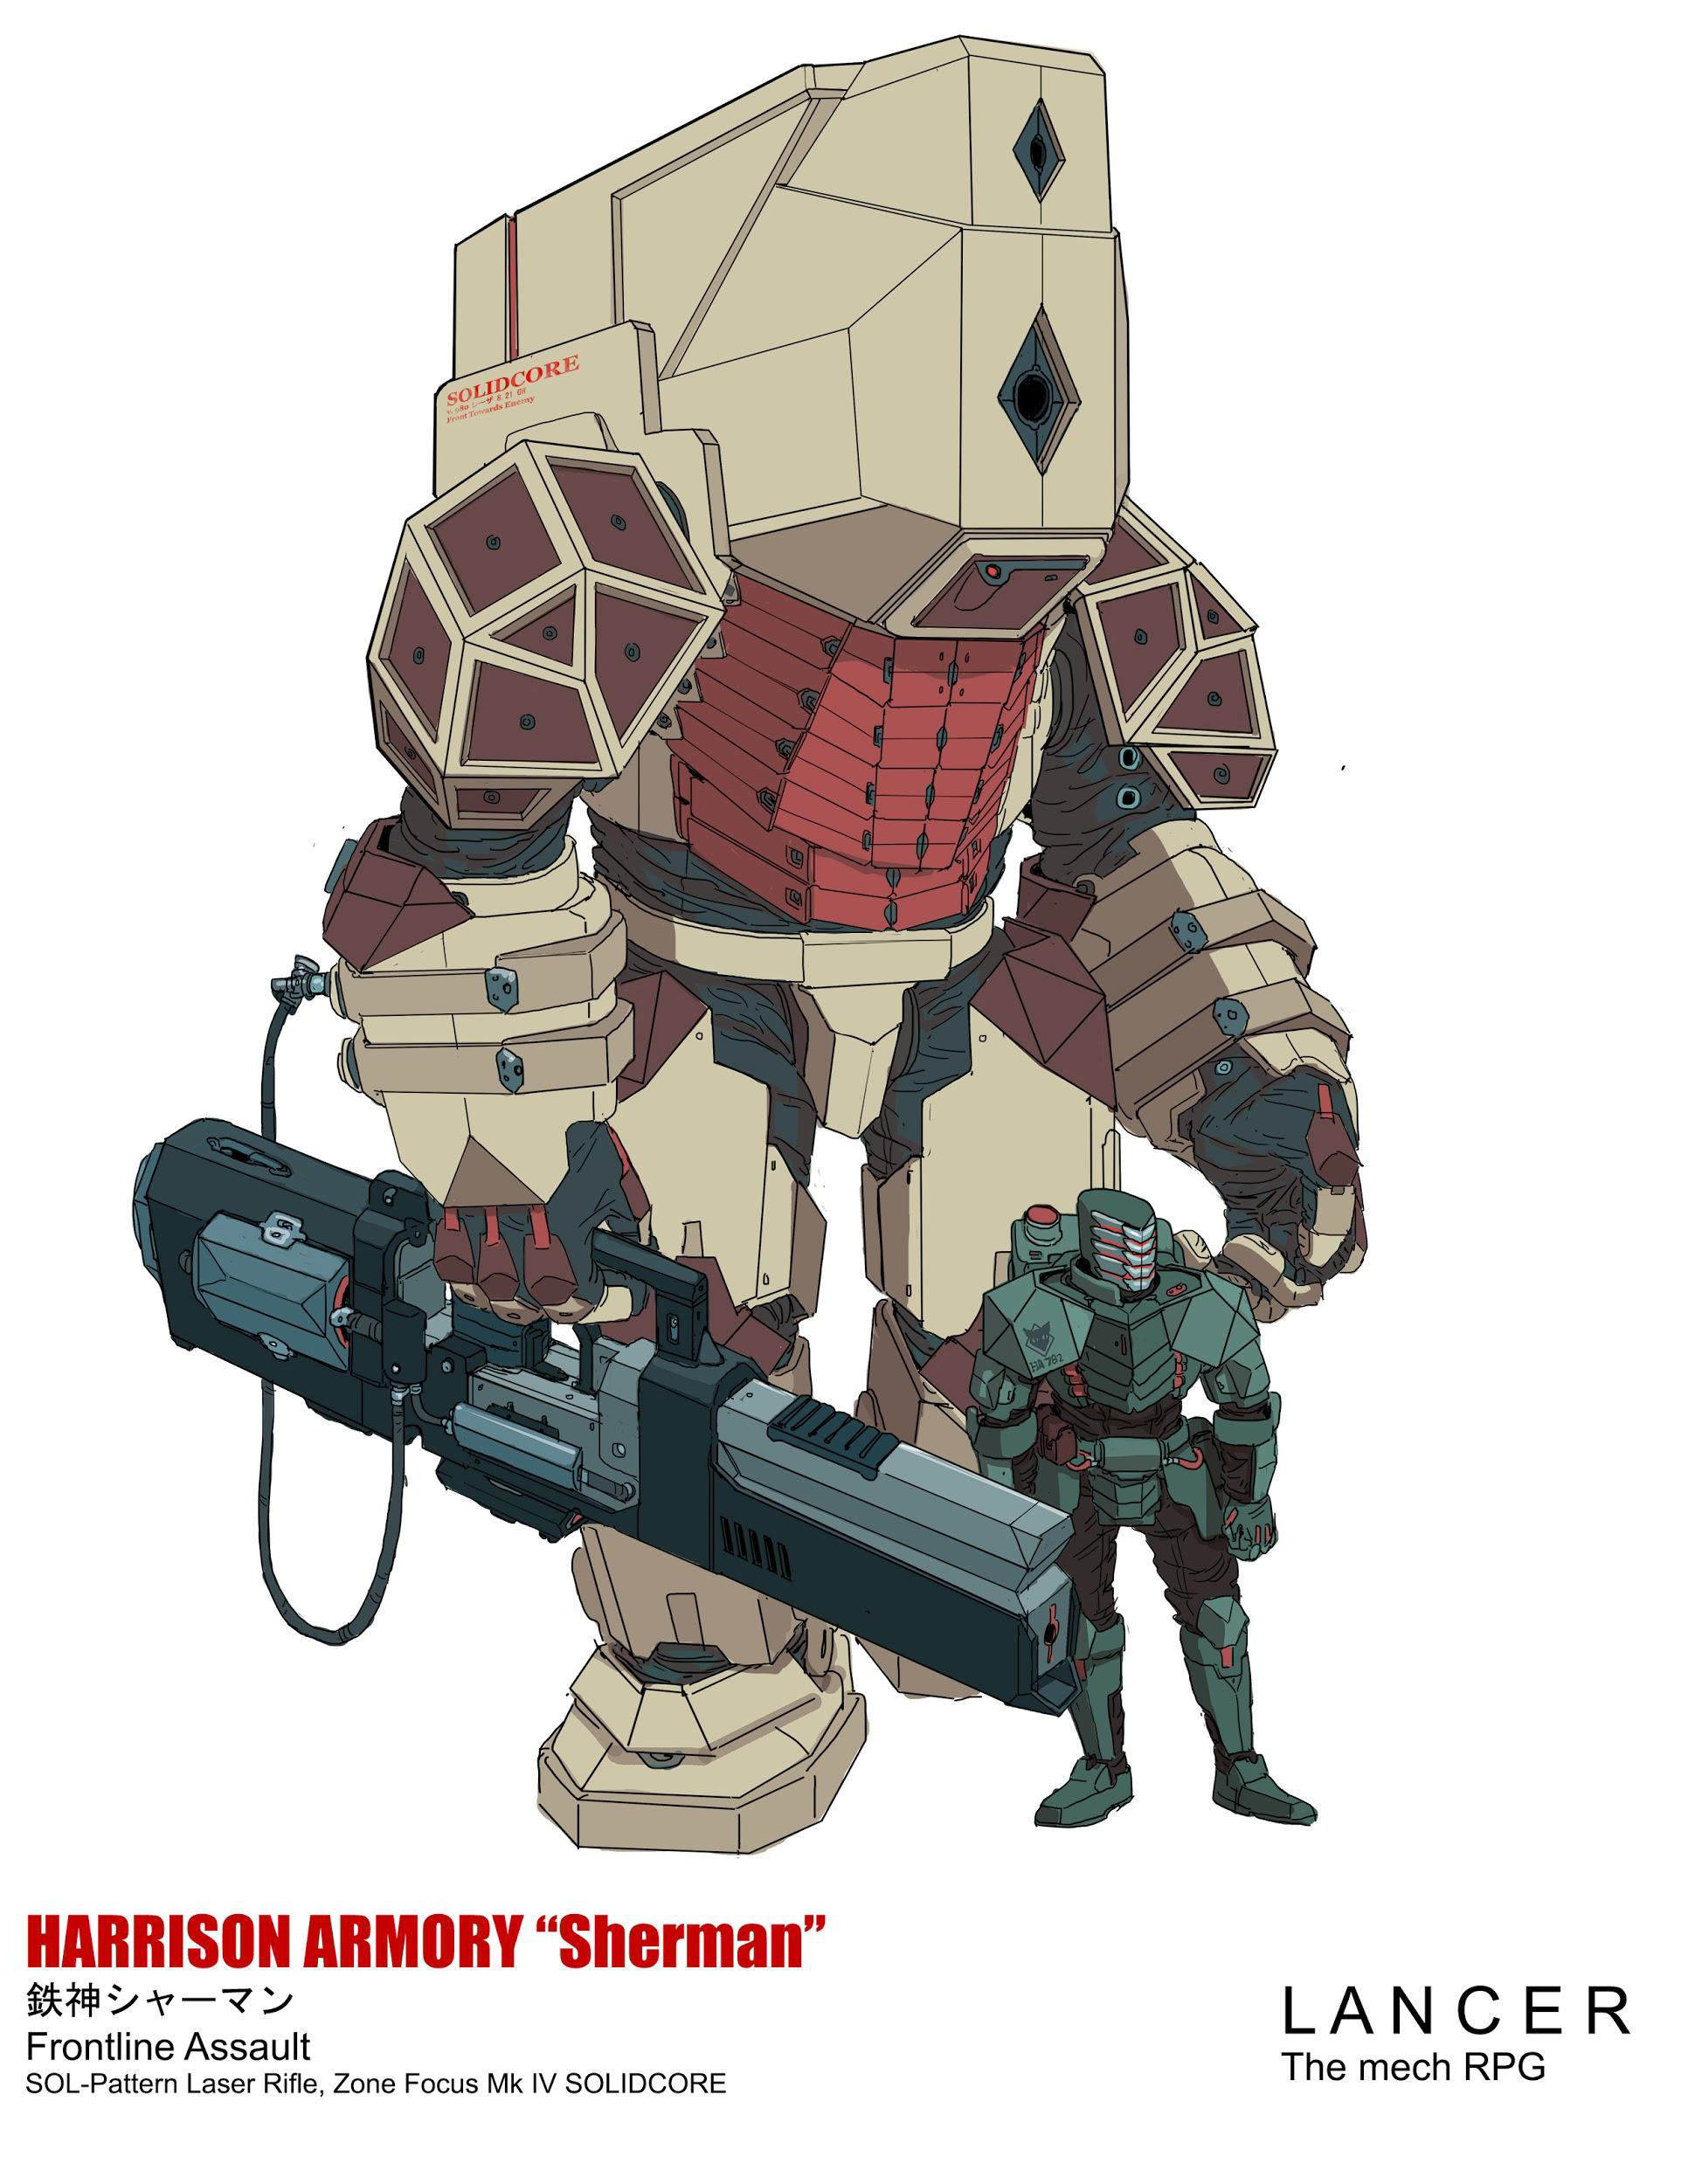
\includegraphics{Sherman}
\end{center}

                              HARRISON ARMORY SHERMAN

The SHERMAN is Harrison Armory‘s line-model chassis: any station, nation, world, stellar, or interstellar

state that holds a fleet-tier contract with Harrison Armory fields a backbone force of localized SHERMAN
cores. The SHERMAN platform is tuned to provide a rugged, versatile power plant for HA‘s fleet-line
energy weaponry and a heat-dispersal system to ensure that the tremendous power requirements do not

overwhelm the chassis‘ tolerance. Next to GMS‘s EVEREST, the SHERMAN is the second most-common
mech chassis in the core systems, so much so that GMS has recently made a push to include more
ablative and wave-scatter defenses into its stock +1 models to deal with hostile actors fielding the

SHERMAN.

                                                  License:

I. Reactor Stabilizer, Laser Rifle

II. SHERMAN FRAME, Heavy Laser, Redundant Systems Upgrade

III. ASURA Class NHP, Tachyon Lance


                                                SHERMAN

 HP: 10         Evasion: 7                            Speed: 3           Heat Cap: 8       Sensors: 10

 Armor: 1       E-Defense: 8                          Size: 1            Repair Cap: 4     Tech Attack:
                                                                                           +0

                                                  TRAITS:

 Superior Reactor: The Sherman has +1 accuracy on engineering checks

 Vent Heat: When the Sherman takes the stabilize action, it counts as in light cover until the start of its
 next turn

                                            SYSTEM POINTS: 5

                                                 MOUNTS:

 Flexible Mount                    Main Mount                            Heavy Mount

                                               CORE system




                                       Zone Focus Mk IV  SOLIDCORE

 The Harrison Armory ZFMk IV SOLIDCORE is a dual-source energy beam weapon hard mounted to a
 chassis. Powered by a milifold power generation system, the ZFMk IV features a secondary belt-fed
 rack of solid-core batteries that can be used to overcharge a single impulse beam, extending the range
 and destructive power of the weapon.

  Integrated Mount: Your mech mounts the ZFMk IV SOLIDCORE, a powerful energy beam weapon.

 SOLIDCORE
  Main Cannon

 Ordnance

  Line 15

  1d3+1 Energy damage


 Active (requires 1 core power): COREBURN Beam

  Full Action

 As a full action, your mech begins to charge this weapon but cannot move or take any other action this
 turn. Your mech stops charging this weapon if it becomes stunned, shut down, jammed, knocked
  prone, or any effect that would cause it to be unable to attack (if it is unable to fire, don’t spend the
 core power). The turn after you start charging this weapon, you may fire it by taking Full Action again.
 Choose a line 30 area originating from your mech. All mechs caught in the area must pass an agility
 check or take 12d6 energy damage, and half on a successful check. Any obstacles or deployables in
 the way are hit automatically and the beam easily penetrates through cover. This beam counts as an
 attack for purposes of systems, talents, etc.

Laser Rifle (SOL-Pattern)

The laser rifle is a near-ubiquitous weapon throughout the galaxy, the energy-based cousin to GMS‘s Type-I
AR. To call it a rifle, though, is shorthand: a laser rifle is a projector that utilizes a series of apertures and
lenses to amplify and focus light into tight beam, visible in the right circumstances, that paints a target long

enough to heat the area of “impact“ into plasma. The HA SOL-pattern laser rifle is capable of a 3.5PW
maximum output, pulsed, but can project a beam at lower power levels; additionally, while some laser rifles
can double as communication/data transfer devices, the Armory‘s SOL is strictly tuned for combat, and has

no such communication capability. The SOL is a solid state and entirely self-contained, but can be patched
into a chassis‘ reactor core for operation and to re-charge spent weaponry. Energy weapons, while having
downsides of their own, are commonly used in micro-and-zero-gravity environments due to having no

impulse or kinetic user feedback.

Main Rifle

Range 10

1 heat (self)

1d6 Energy Damage + Burn 1


Reactor Stabilizer

A necessary component of most energy-based mechs, reactor stabilizers add another layer of failsafe
protocols to vent heat, manage power flow, and shunt excessive output into weapons and systems in need.

3 SP, Unique




When you gain a point of reactor stress, you can re-roll your overheating check (but must keep
the second result, even if it’s worse).


Heavy Laser

A heavy laser rifle is a larger-scale laser weapon. The Harrison Armory ANDROMEDA-pattern heavy laser
scales up the SOL by half, adding a second projector that can fire independently, synchronized, or in

alternating patterns and wavelengths as the primary projector. The effect overwhelms most shields, but the
power draw necessary makes this weapon impractical on platforms without the necessary heat reduction/

dispersal to manage the incredible cost.

Heavy Cannon

3 heat (self)

Range 15

2d6 energy damage + Burn 3


Redundant Systems upgrade

A common right-of-distribution modification by pilots in forward operating bases, building further
redundancy into a chassis‘s systems guarantees a measure of reliability beyond stock design standards.

2 SP, Unique, Limited (1)
You can activate this module to make a Stabilize action as a quick action.


ASURA-class NHP

ASURA was born from the Armory‘s Think Tank thought-war games as a response to repeated failures

during a forlorn hope scenario test; ASURA manifested in simulated mechs‘ systems as a recode of
HORUS‘s PUPPETMASTER virus, hijacking friendly cores and forcing them into action far beyond human
capacity -- action at speed and intensity that the registered g-force caused the sim-pilots to die, suffocated

and crushed by the sudden amplified mass of their own bodies.

While such results were initially deemed a failure by Think Tank NHPs and engineers, further study on

ASURA was commissioned. Personality and parasentience code was injected into the initial anomalous
PUPPETMASTER, first contact handled by Think Tank NHPs, and societal acclimation and conditioning
was fast tracked, giving Armory engineers the first iteration of ASURA after roughly a decade of study, re-

coding, and reeducation. ASURA, as it exists now, is a scaled-back version of that initial manifestation:
while retaining some of its initial alacratic impulse, ASURA now recognizes the need to keep its pilot alive,
and will operate within parameters set by its pilot‘s medical and psychological tolerances.

3 SP, Unique

AI

Your mech gains the AI property and the ASURA protocol:

         ASURA protocol
	        Protocol

         Limited (1)





         This turn only, gain an extra two quick actions or one full action. These extra actions must
         still obey normal rules about duplicating actions (you can’t use it to Boost if you’ve
         already Boosted this turn, for example

         This protocol can only be activated once per scene.


Tachyon Lance

The tachyon lance is the weaponized result of early Harrison Armory experiments into faster-than-light
travel. Rendered obsolete by developments in blinkspace travel and the difficulty of ensuring corporeal

passenger survival, HA‘s tachyon accelerators were mothballed until Think Tank engineers realized their
potential application as weapons. A tachyon accelerator projects tachyon particles -- essentially a
subatomic localized object -- faster than light towards its target. These particles are impossible to see

through optical/visible means: as they travel faster than light, they cannot be seen or avoided intentionally.
Though the size of the particle is tiny, the sheer speed and energy of travel is titanic, and the damage a
tachyon lance imparts on its target -- should it connect -- is unparalleled.

Superheavy Cannon

Ordnance, 4 heat (self)

Range 20, Burn 8

2d6 Energy damage

